% A BLAKE3 chunk [BLAKE3, §2.4]: up to 16 blocks of 64 bytes, compressed in order from the key
% words with counter t = chunk index; the first block sets CHUNK_START, the last CHUNK_END (and
% ROOT if the chunk is the whole tree). The last block may be short and is zero-padded.
% Original drawing for the Hash library.
\documentclass[tikz,border=6pt]{standalone}
\usepackage[T1]{fontenc}
\usepackage{lmodern}
% Shared style for the Hash diagrams.
% Palette: Okabe–Ito (colour-blind safe). Every diagram is drawn on an opaque white card so it
% stays legible on dark page themes.
\usetikzlibrary{arrows.meta,positioning,calc,fit,backgrounds}
\definecolor{hsblue}{HTML}{0072B2}
\definecolor{hsorange}{HTML}{E69F00}
\definecolor{hsgreen}{HTML}{009E73}
\definecolor{hsvermilion}{HTML}{D55E00}
\definecolor{hspurple}{HTML}{CC79A7}
\definecolor{hsink}{HTML}{1F2933}
\tikzset{
  >={Stealth[length=2.2mm]},
  every node/.style={font=\sffamily\small, text=hsink},
  wire/.style={draw=hsink, line width=0.6pt, ->},
  reg/.style={draw=hsink, line width=0.6pt, fill=hsblue!12, minimum width=9mm, minimum height=7mm},
  fn/.style={draw=hsink, line width=0.6pt, fill=hsorange!25, rounded corners=2pt, minimum width=10mm, minimum height=6mm},
  input/.style={draw=hsink, line width=0.6pt, fill=hsgreen!20, minimum width=9mm, minimum height=6mm},
  add/.style={circle, draw=hsink, line width=0.6pt, fill=white, inner sep=0pt, minimum size=5mm, font=\sffamily\bfseries},
  card/.style={fill=white, rounded corners=4pt},
}

\begin{document}
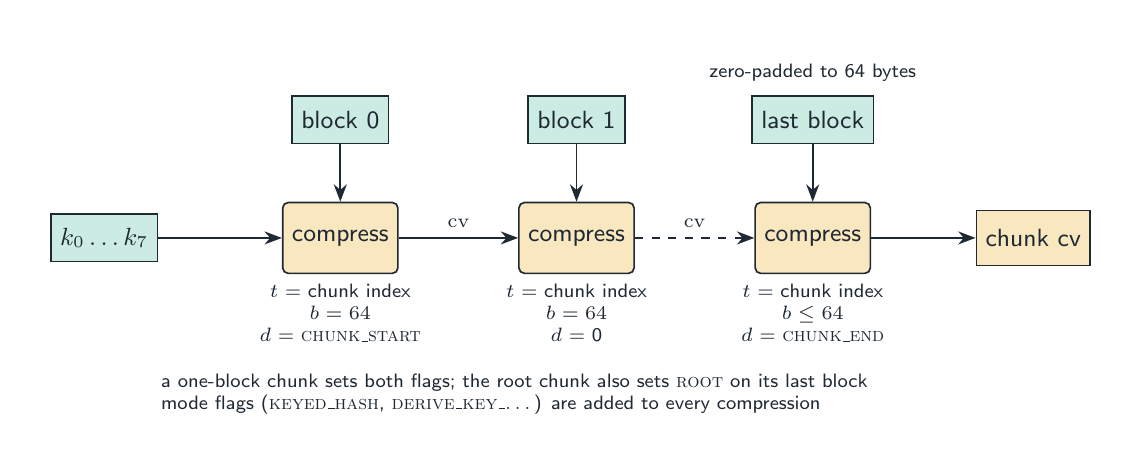
\begin{tikzpicture}
  \def\dx{3.0}
  \node[input, fill=hsgreen!20] (k) at (0,0) {$k_0 \ldots k_7$};
  \foreach \i/\lbl/\b/\d in {1/{block 0}/{b = 64}/{\textsc{chunk\_start}}, 2/{block 1}/{b = 64}/{0},
      3/{last block}/{b \le 64}/{\textsc{chunk\_end}}} {
    \node[fn, minimum width=13mm, minimum height=9mm] (F\i) at (\i*\dx, 0) {compress};
    \node[input] (B\i) at (\i*\dx, 1.5) {\lbl};
    \draw[wire] (B\i) -- (F\i);
    \node[font=\sffamily\scriptsize, anchor=north, align=center] at (F\i.south)
      {$t$ = chunk index\\$\b$\\$d$ = \d};
  }
  \draw[wire] (k) -- (F1);
  \draw[wire] (F1) -- node[above, font=\scriptsize] {cv} (F2);
  \draw[wire, dashed] (F2) -- node[above, font=\scriptsize] {cv} (F3);
  \node[reg, fill=hsorange!25] (cv) at (4*\dx - 0.2, 0) {chunk cv};
  \draw[wire] (F3) -- (cv);
  \node[font=\sffamily\scriptsize, anchor=south, align=center] at ($(B3.north)+(0,0.05)$)
    {zero-padded to 64 bytes};
  \node[font=\sffamily\scriptsize, anchor=north west, align=left] at (0.6,-1.6)
    {a one-block chunk sets both flags; the root chunk also sets \textsc{root} on its last block\\
     mode flags (\textsc{keyed\_hash}, \textsc{derive\_key\_\ldots}) are added to every compression};
  \begin{scope}[on background layer]
    \coordinate (e1) at (-0.9,-2.5);
    \coordinate (e2) at (4*\dx+0.7,2.6);
    \node[card, fit=(e1)(e2), inner sep=2pt] {};
  \end{scope}
\end{tikzpicture}
\end{document}
